% ═══════════════════════════════════════════════════════════════════
% ops-knowledge-loop — Ember Grid
% LaTeX Beamer source — fully dark projector-style PDF
%
% BUILD (22 slides: 14 main + 8 appendix — matches slides_content.md):
%   cd pdf/beamer
%   tectonic presentation.tex --outdir=..
%   mv ../presentation.pdf ../presentation.beamer.pdf
% Or with xelatex (two passes for refs):
%   xelatex -output-directory=../ presentation.tex && xelatex -output-directory=../ presentation.tex
%   mv ../presentation.pdf ../presentation.beamer.pdf
%
% EDIT THESE TWO LINES BEFORE YOUR DEMO / INTERVIEW:
\newcommand{\demodays}{[X days]}        % ← FILL IN
\newcommand{\demorole}{[Role Name]}     % ← FILL IN
% ═══════════════════════════════════════════════════════════════════

\documentclass[aspectratio=169,10pt]{beamer}

% ── Metropolis theme (install: tlmgr install beamertheme-metropolis)
\usetheme[progressbar=frametitle,block=fill]{metropolis}

% ── XeTeX font loading
\usepackage{fontspec}
\setmainfont{DejaVu Sans}[Scale=1.0]
\setmonofont{DejaVu Sans Mono}[Scale=0.88]
% If JetBrains Mono is installed, replace with:
% \setmonofont{JetBrains Mono}[Scale=0.88]

\usepackage{xcolor}
\usepackage{booktabs}
\usepackage{tabularx}
\usepackage{colortbl}
\usepackage{array}
\usepackage{tikz}
\usepackage{graphicx}
\usepackage{ragged2e}

% ── DESIGN TOKENS ─────────────────────────────────────────────────
\definecolor{bgdark}{HTML}{0A0F0A}
\definecolor{bgdark2}{HTML}{0F1A0F}
\definecolor{bgdark3}{HTML}{162016}
\definecolor{cgreen}{HTML}{00FF41}
\definecolor{cgreenD}{HTML}{00CC33}
\definecolor{cteal}{HTML}{19E6C5}
\definecolor{camber}{HTML}{FFC857}
\definecolor{ctext}{HTML}{C8E6C9}
\definecolor{cdim}{HTML}{6B8F6B}
\definecolor{cborder}{HTML}{1E3A1E}
\definecolor{cauto}{HTML}{00AA2B}
\definecolor{cpend}{HTML}{CC9F40}
\definecolor{cterm}{HTML}{90EE90}

% ── METROPOLIS COLOUR OVERRIDES ───────────────────────────────────
\setbeamercolor{normal text}{fg=ctext,bg=bgdark}
\setbeamercolor{alerted text}{fg=cgreen}
\setbeamercolor{example text}{fg=cteal}
\setbeamercolor{frametitle}{bg=bgdark2,fg=cgreen}
\setbeamercolor{progress bar}{fg=cgreen,bg=bgdark3}
\setbeamercolor{block title}{bg=bgdark2,fg=cgreen}
\setbeamercolor{block body}{bg=bgdark3,fg=ctext}
\setbeamercolor{structure}{fg=cgreen}
\setbeamercolor{background canvas}{bg=bgdark}
\setbeamercolor{footline}{fg=cdim,bg=bgdark2}

% ── TYPOGRAPHY TWEAKS ─────────────────────────────────────────────
\setbeamerfont{frametitle}{size=\large,series=\bfseries,family=\ttfamily}
\setbeamerfont{title}{size=\Huge,series=\bfseries,family=\ttfamily}
\setbeamerfont{subtitle}{size=\normalsize}
\setbeamerfont{normal text}{size=\small}
\renewcommand{\baselinestretch}{1.2}

% ── BULLET STYLE ──────────────────────────────────────────────────
\setbeamertemplate{itemize item}{\color{cgreen}{\small$\triangleright$}}
\setbeamertemplate{itemize subitem}{\color{cteal}{\footnotesize$\triangleright$}}

% ── STATUS FOOTLINE ───────────────────────────────────────────────
\setbeamertemplate{footline}{%
  \leavevmode%
  \hbox{\begin{beamercolorbox}[wd=\paperwidth,ht=14pt,dp=4pt]{footline}%
    \hspace{0.5cm}%
    {\color{cgreen}\ttfamily\scriptsize ember@ops:~\$}%
    \hspace{0.3cm}%
    {\color{cdim}\ttfamily\scriptsize slide \insertframenumber/\inserttotalframenumber}%
    \hfill%
    {\color{cdim}\ttfamily\scriptsize ops-knowledge-loop · Ember Grid}%
    \hspace{0.5cm}%
  \end{beamercolorbox}}%
}

% ── HELPERS ───────────────────────────────────────────────────────
\newcommand{\slidecat}[1]{{\color{cdim}\ttfamily\scriptsize\MakeUppercase{#1}}}

\newcolumntype{L}[1]{>{\RaggedRight\arraybackslash}p{#1}}

% Confidence bar using tikz
\newcommand{\confbar}[2]{%
  % #1 = value 0-1, #2 = color
  \tikz[baseline=-0.5ex]{
    \fill[bgdark3] (0,0) rectangle (2.2cm,4pt);
    \fill[#2]      (0,0) rectangle (#1*2.2cm,4pt);
  }%
}

\newcommand{\autochip}[1]{%
  \fcolorbox{cauto}{bgdark2}{%
    {\color{cauto}\ttfamily\tiny\bfseries #1}%
  }%
}
\newcommand{\pendchip}[1]{%
  \fcolorbox{cpend}{bgdark2}{%
    {\color{cpend}\ttfamily\tiny\bfseries #1}%
  }%
}

\newenvironment{terminal}{%
  \begin{beamercolorbox}[sep=6pt,rounded=true,shadow=false]{block body}%
  \ttfamily\tiny\color{cterm}%
}{%
  \end{beamercolorbox}%
}

% ══════════════════════════════════════════════════════════════════
\begin{document}

% ── TITLE PAGE ────────────────────────────────────────────────────
{
\setbeamercolor{background canvas}{bg=bgdark}
\begin{frame}[plain]
  \vspace{1.2cm}
  \slidecat{ops-knowledge-loop}
  \vspace{0.3cm}

  {\color{cgreen}\ttfamily\Huge\bfseries ops-knowledge-loop}

  \vspace{0.3cm}
  {\color{cteal}\large AI-Powered Incident Triage · Ember Grid}

  \vspace{0.2cm}
  {\color{cdim}\ttfamily\small $\triangleright$ From alert to remediation in under 2 minutes}

  \vspace{0.8cm}
  \begin{beamercolorbox}[sep=6pt,rounded=true]{block body}
    {\color{cgreenD}\ttfamily\footnotesize
    INCIDENT $\rightarrow$ RAG $\rightarrow$ LLM $\rightarrow$ GATE $\rightarrow$ RUNDECK $\rightarrow$ TICKET CLOSED}
  \end{beamercolorbox}
\end{frame}
}

% ── SLIDE 2: PRIOR ART ────────────────────────────────────────────
\newcommand{\priorbox}[2]{%
  \begin{beamercolorbox}[wd=\linewidth,sep=0pt,rounded=false,shadow=false]{block body}%
    {\color{#1}\ttfamily\tiny\bfseries #2}\\[-0.1em]
    \rule{\linewidth}{0.4pt}\\[0.15em]
}
\newcommand{\priorboxend}{\end{beamercolorbox}}
\newcommand{\priortagline}[1]{%
  \par\vspace{0.04cm}%
  {\color{cdim}\fontsize{5}{5.5}\selectfont\itshape%
   \linespread{0.75}\selectfont%
   \parbox[t]{\linewidth}{\raggedright\arraybackslash\setlength{\parskip}{0pt}#1}}%
}

\begin{frame}{Prior Art}
  \slidecat{Background}
  {\color{cdim}\small Three projects that map directly onto this one.}
  \vspace{0.12cm}
  \begin{columns}[T,onlytextwidth]
    \begin{column}{0.31\textwidth}
      \priorbox{cgreen}{┌─ WOLF FRAMEWORK ─────────────────┐}
      {\color{cgreen}\ttfamily\tiny\bfseries LangChain · ChromaDB · MCP · local LLM}\\[0.08cm]
      {\color{ctext}\ttfamily\scriptsize\bfseries WOLF Framework}\\[0.04cm]
      {\color{cdim}\tiny Open-source AI-assisted game dev · 2025--present}\\[0.1cm]
      {\color{ctext}\tiny
      \begin{itemize}\setlength\itemsep{1pt}
        \item LangChain + ChromaDB + LiteLLM RAG via MCP
        \item Headless SimBot: evidence-gate-action loop
        \item Local (Ollama) and cloud/paid variants
      \end{itemize}}
      \priortagline{Same RAG stack and architectural pattern as this project.}
      \priorboxend
    \end{column}
    \begin{column}{0.31\textwidth}
      \priorbox{cteal}{┌─ QVC / QURATE RETAIL ────────────┐}
      {\color{cteal}\ttfamily\tiny\bfseries \textasciitilde850 services · 5y zero audit breach}\\[0.08cm]
      {\color{ctext}\ttfamily\scriptsize\bfseries Cloud Migration}\\[0.04cm]
      {\color{cdim}\tiny \textasciitilde850 K8s microservices · 2020--2024}\\[0.1cm]
      {\color{ctext}\tiny
      \begin{itemize}\setlength\itemsep{1pt}
        \item Migrated off Jenkins, Spinnaker, Rancher, Bitbucket, Ansible fully to Azure DevOps
        \item Live multi-DC AEM deployments; up to 40 stakeholders
        \item Zero audit breach over 5 years; ServiceNow tracked
      \end{itemize}}
      \priortagline{Same retail-scale infrastructure, ServiceNow, and gating discipline.}
      \priorboxend
    \end{column}
    \begin{column}{0.31\textwidth}
      \priorbox{camber}{┌─ MULTI-GEO MOBILE PIPELINE ──────┐}
      {\color{camber}\ttfamily\tiny\bfseries Release: 3h $\rightarrow$ 30min}\\[0.04cm]
      {\color{camber}\ttfamily\tiny\bfseries PR acceptance: 2h $\rightarrow$ 20min}\\[0.08cm]
      {\color{ctext}\ttfamily\scriptsize\bfseries Build-Test-Deploy}\\[0.04cm]
      {\color{cdim}\tiny Bitbucket · Jenkins · Artifactory · Jira · Consul}\\[0.1cm]
      {\color{ctext}\tiny
      \begin{itemize}\setlength\itemsep{1pt}
        \item Multi-geo mobile build-test-deploy pipeline
        \item Release effort: 3 hours $\rightarrow$ 30 minutes
        \item Automated PR acceptance: 2 hours $\rightarrow$ 20 minutes
        \item Stage tracking, drift detection, rollback paths
      \end{itemize}}
      \priortagline{Same compression pattern applied to incident response.}
      \priorboxend
    \end{column}
  \end{columns}
  \vspace{0.1cm}
  {\color{cdim}\ttfamily\tiny $\triangleright$ 8+ years automotive \& UK retail · Ansible · ServiceNow · multi-geo release engineering · RAG / MCP / local-LLM}
\end{frame}

% ── SLIDE 3: THE PROBLEM ──────────────────────────────────────────
\begin{frame}{The On-Call Problem}
  \slidecat{Context}
  \vspace{0.2cm}
  \begin{block}{\color{cgreen}\ttfamily\small MEAN TIME TO REMEDIATION}
    Mean time to remediation is dominated by \textit{lookup time}, not fix time
  \end{block}
  \vspace{0.15cm}
  \begin{block}{\color{cteal}\ttfamily\small KNOWLEDGE SILO}
    Institutional knowledge lives in engineers' heads, not in systems
  \end{block}
  \vspace{0.15cm}
  \begin{block}{\color{camber}\ttfamily\small REPEAT WORK}
    Repeated incidents get manually triaged every single time
  \end{block}
  \vspace{0.3cm}
  {\color{cdim}\ttfamily\small $\triangleright$ Ember Grid runs 17 microservices across UK retail infrastructure}
\end{frame}

% ── SLIDE 3: ARCHITECTURE ─────────────────────────────────────────
\begin{frame}{How It Works}
  \slidecat{Architecture}
  \vspace{0.3cm}
  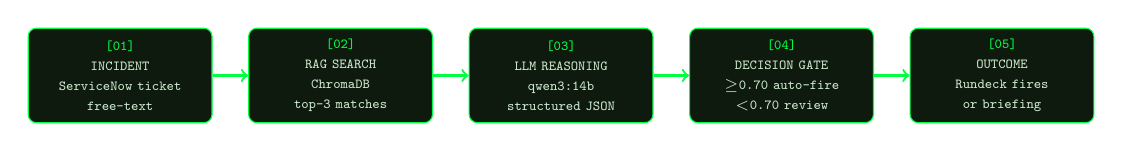
\begin{tikzpicture}[
    stage/.style={
      rectangle, draw=cgreen, fill=bgdark2, text=ctext,
      rounded corners=3pt, minimum height=1.2cm,
      text width=2.1cm, align=center, font=\ttfamily\tiny
    },
    arrow/.style={->, color=cgreen, thick}
  ]
    \node[stage] (s1) at (0,0) {{\color{cgreen}\bfseries[01]}\\\textbf{INCIDENT}\\ServiceNow ticket\\free-text};
    \node[stage] (s2) at (2.8,0) {{\color{cgreen}\bfseries[02]}\\\textbf{RAG SEARCH}\\ChromaDB\\top-3 matches};
    \node[stage] (s3) at (5.6,0) {{\color{cgreen}\bfseries[03]}\\\textbf{LLM REASONING}\\qwen3:14b\\structured JSON};
    \node[stage] (s4) at (8.4,0) {{\color{cgreen}\bfseries[04]}\\\textbf{DECISION GATE}\\ $\geq$0.70 auto-fire\\$<$0.70 review};
    \node[stage] (s5) at (11.2,0) {{\color{cgreen}\bfseries[05]}\\\textbf{OUTCOME}\\Rundeck fires\\or briefing};
    \draw[arrow] (s1.east) -- (s2.west);
    \draw[arrow] (s2.east) -- (s3.west);
    \draw[arrow] (s3.east) -- (s4.west);
    \draw[arrow] (s4.east) -- (s5.west);
  \end{tikzpicture}

  \vspace{0.4cm}
  \begin{beamercolorbox}[sep=5pt,rounded=true,wd=\textwidth]{alerted text}
    {\color{cgreen}\ttfamily\small $\triangleright$ Fully local · No data leaves the machine · No API costs · \textasciitilde30s end-to-end}
  \end{beamercolorbox}
\end{frame}

% ── SLIDE 4: KNOWLEDGE BASE ───────────────────────────────────────
\begin{frame}{What the RAG Searches}
  \slidecat{Data}
  \vspace{0.2cm}
  \begin{columns}[T]
    \begin{column}{0.48\textwidth}
      {\color{cteal}\ttfamily\small\bfseries $\triangleright$ INCIDENT HISTORY}
      \vspace{0.1cm}
      \begin{itemize}\itemsep2pt
        \item 500+ synthetic incidents across 17 services
        \item Each indexed as a vector embedding in ChromaDB
        \item {\color{cdim}\ttfamily\tiny OOM kills · latency spikes · ETL failures · EDI mismatches · POS outages · loyalty bugs · notification duplicates}
      \end{itemize}
    \end{column}
    \begin{column}{0.48\textwidth}
      {\color{cteal}\ttfamily\small\bfseries $\triangleright$ RUNBOOKS}
      \vspace{0.1cm}
      \begin{itemize}\itemsep2pt
        \item Per-service markdown runbooks
        {\color{cdim}\ttfamily\tiny checkout · product-search · payment-processor · \ldots}
        \item Auto-generated runbooks from resolved ServiceNow tickets
        \item Chunked and embedded alongside incident history
      \end{itemize}
    \end{column}
  \end{columns}
  \vspace{0.3cm}
  \rule{\textwidth}{0.3pt}
  {\color{cdim}\ttfamily\tiny
    All embeddings: {\color{cteal}\bfseries all-MiniLM-L6-v2} · Similarity threshold: {\color{cgreen}\bfseries 0.60} strong match}
\end{frame}

% ── SLIDE 5: DASHBOARD ────────────────────────────────────────────
\begin{frame}{Ops Dashboard}
  \slidecat{Tooling}
  \vspace{0.2cm}
  \begin{columns}[T]
    \begin{column}{0.5\textwidth}
      \begin{itemize}\itemsep3pt
        \item Recent incidents and their triage status
        \item RAG match scores per incident
        \item AI recommendation with confidence score
        \item Decision gate outcome (auto-executed vs pending review)
        \item Rundeck job catalogue
      \end{itemize}
      \vspace{0.2cm}
      \fcolorbox{cteal}{bgdark2}{{\color{cteal}\ttfamily\small Flask · localhost:5000}}
    \end{column}
    \begin{column}{0.44\textwidth}
      \begin{terminal}
ops-knowledge-loop dashboard\\
+------+--------------+--------+\\
\textbar{} INC  \textbar{} STATUS       \textbar{} CONF   \textbar{}\\
+------+--------------+--------+\\
\textbar{} 0043 \textbar{} AUTO-EXECUTE \textbar{} 0.95 v \textbar{}\\
\textbar{} 0044 \textbar{} PENDING      \textbar{} 0.35 \textasciitilde{} \textbar{}\\
\textbar{} 0045 \textbar{} AUTO-EXECUTE \textbar{} 0.75 v \textbar{}\\
+------+--------------+--------+\\
      \end{terminal}
    \end{column}
  \end{columns}
\end{frame}

% ── SLIDE 6: LIVE DEMO RESULTS ────────────────────────────────────
\begin{frame}{10 Queries · Live Run}
  \slidecat{Results}
  \vspace{0.1cm}
  \hspace{0.2cm}
  \fcolorbox{cauto}{bgdark3}{{\color{cauto}\ttfamily\normalsize\bfseries 5} {\color{cauto}\ttfamily\tiny AUTO-EXECUTED}}
  \hspace{0.4cm}
  \fcolorbox{cpend}{bgdark3}{{\color{cpend}\ttfamily\normalsize\bfseries 5} {\color{cpend}\ttfamily\tiny PENDING REVIEW}}
  \hfill
  {\color{cdim}\ttfamily\tiny gate: 0.70}
  \vspace{0.15cm}

  {\tiny
  \begin{tabularx}{\textwidth}{@{}L{3.1cm}L{3.5cm}L{2.2cm}L{2.4cm}@{}}
    \toprule
    {\color{cgreen}\ttfamily INCIDENT} &
    {\color{cgreen}\ttfamily RECOMMENDED JOB} &
    {\color{cgreen}\ttfamily CONFIDENCE} &
    {\color{cgreen}\ttfamily OUTCOME} \\
    \midrule
    \rowcolor{bgdark2}
    checkout-service OOM kill & restart-service-with-memory-bump & \confbar{0.95}{cauto}~0.95 & \autochip{AUTO-EXECUTE} \\
    \rowcolor{bgdark3}
    payment-processor 500 errors & rollback-to-previous-version & \confbar{0.95}{cauto}~0.95 & \autochip{AUTO-EXECUTE} \\
    \rowcolor{bgdark2}
    product-search unresponsive & reindex-elasticsearch & \confbar{0.75}{cauto}~0.75 & \autochip{AUTO-EXECUTE} \\
    \rowcolor{bgdark3}
    inventory sync stalled & force-inventory-sync & \confbar{0.66}{cpend}~0.66 & \pendchip{PENDING REVIEW} \\
    \rowcolor{bgdark2}
    store POS tills unresponsive & rollback-to-previous-version & \confbar{0.75}{cauto}~0.75 & \autochip{AUTO-EXECUTE} \\
    \rowcolor{bgdark3}
    loyalty svc not awarding pts & restart-service-rolling & \confbar{0.35}{cpend}~0.35 & \pendchip{PENDING REVIEW} \\
    \rowcolor{bgdark2}
    order fulfilment latency spike & scale-up-replicas & \confbar{0.75}{cauto}~0.75 & \autochip{AUTO-EXECUTE} \\
    \rowcolor{bgdark3}
    notification svc dup emails & restart-service-with-memory-bump & \confbar{0.35}{cpend}~0.35 & \pendchip{PENDING REVIEW} \\
    \rowcolor{bgdark2}
    supplier EDI orders dropped & force-inventory-sync & \confbar{0.65}{cpend}~0.65 & \pendchip{PENDING REVIEW} \\
    \rowcolor{bgdark3}
    recommendation engine degraded & reindex-elasticsearch & \confbar{0.45}{cpend}~0.45 & \pendchip{PENDING REVIEW} \\
    \bottomrule
  \end{tabularx}
  }
  \vspace{0.1cm}
  {\color{cdim}\ttfamily\tiny ``The gate is discriminating by design — weak RAG similarity or ambiguous root cause correctly suppresses auto-execution''}
\end{frame}

% ── FEATURED TERMINAL SLIDES Q1, Q3, Q6 ───────────────────────────

\begin{frame}{Q1 — checkout-service OOM kill}
  \slidecat{Live Output — Query 1 / 10}
  {\color{cteal}\ttfamily\small\bfseries confidence 0.95 -> AUTO-EXECUTE}
  \vspace{0.15cm}
  \begin{terminal}
    \$ python query\_live.py ``checkout service OOM kill, container hitting memory limit and restarting repeatedly under load''\\
    \vspace{0.25em}
    RAG Top 3:\\
    \hspace*{0.4cm}1  incidents.json  0.797 ✓ strong match  [INC0043096] checkout-service OOM kill\\
    \hspace*{0.4cm}2  incidents.json  0.796 ✓ strong match  [INC0043144] checkout-service OOM kill\\
    \hspace*{0.4cm}3  incidents.json  0.795 ✓ strong match  [INC0043048] checkout-service OOM kill\\
    \vspace{0.25em}
    ✓ Strong precedent found — incidents.json (similarity 0.797)\\
    \vspace{0.25em}
    Recommended Job : {\color{cauto}restart-service-with-memory-bump}\\
    Confidence      : {\color{cauto}0.95}  |  Gate: {\color{cauto}AUTO-EXECUTE}\\
    Reasoning       : OOM kills due to memory limits directly align with the job purpose.\\
    \hspace*{0.4cm}Runbook context explicitly confirms memory threshold breach as trigger.\\
    \vspace{0.25em}
    {\color{cauto}✓ WOULD AUTO-EXECUTE  —  restart-service-with-memory-bump  (confidence 0.95 ≥ 0.70 gate)}\\
    Total runtime: 8.7s
  \end{terminal}
\end{frame}

\begin{frame}{Q3 — product-search unresponsive after deploy}
  \slidecat{Live Output — Query 3 / 10}
  {\color{cteal}\ttfamily\small\bfseries confidence 0.75 -> AUTO-EXECUTE}
  \vspace{0.15cm}
  \begin{terminal}
    \$ python query\_live.py ``product search returning empty results, search index unresponsive after deployment''\\
    \vspace{0.25em}
    RAG Top 3:\\
    \hspace*{0.4cm}1  product-search.md  0.575 \textasciitilde{} partial  Service Overview: ES-backed search service\\
    \hspace*{0.4cm}2  incidents.json     0.571 \textasciitilde{} partial  [INC0043346] product-search slow query (1352ms)\\
    \hspace*{0.4cm}3  product-search.md  0.570 \textasciitilde{} partial  Diagnostic Steps: kubectl exec cache hit rate\\
    \vspace{0.25em}
    ⚠ No close precedent — best match 0.575 in product-search.md. AI will deduce a remediation.\\
    \vspace{0.25em}
    Recommended Job : {\color{cauto}reindex-elasticsearch}\\
    Confidence      : {\color{cauto}0.75}  |  Gate: {\color{cauto}ABOVE GATE -> AUTO-EXECUTE}\\
    Reasoning       : Unresponsive ES index directly maps to reindexing as remediation step.\\
    \hspace*{0.4cm}Runbook + incident context both confirm the service architecture.\\
    \vspace{0.25em}
    {\color{cauto}✓ WOULD AUTO-EXECUTE  —  reindex-elasticsearch  (confidence 0.75 ≥ 0.70 gate)}\\
    Total runtime: 9.9s
  \end{terminal}
\end{frame}

\begin{frame}{Q6 — loyalty service not awarding points}
  \slidecat{Live Output — Query 6 / 10}
  {\color{camber}\ttfamily\small\bfseries confidence 0.35 -> PENDING REVIEW}
  \vspace{0.15cm}
  \begin{terminal}
    \$ python query\_live.py ``loyalty service not awarding points after purchase, customer accounts not updating''\\
    \vspace{0.25em}
    RAG Top 3:\\
    \hspace*{0.4cm}1  incidents.json  0.642 \textasciitilde{} partial  [INC0042145] loyalty-service failing to award points\\
    \hspace*{0.4cm}\hspace*{0.4cm}(click-and-collect, missing order type mapping)\\
    \hspace*{0.4cm}2  incidents.json  0.562 \textasciitilde{} partial  [INC0041652] reward redemption 500 (DB pool exhausted)\\
    \hspace*{0.4cm}3  incidents.json  0.561 \textasciitilde{} partial  [INC0041134] points returning negatives (bulk redemption)\\
    \vspace{0.25em}
    ⚠ No close precedent — best match 0.642. AI will deduce a remediation.\\
    \vspace{0.25em}
    Recommended Job : {\color{camber}restart-service-rolling}\\
    Confidence      : {\color{camber}0.35  <-- MODEL SELF-DOWNGRADED}  |  Gate: {\color{camber}RULE-BASED FALLBACK}\\
    Reasoning       : Past loyalty-service issues resolved via restarts or config updates.\\
    \hspace*{0.4cm}Runbook context references backfill scripts — not a restart path.\\
    \hspace*{0.4cm}Semantic mismatch between query and available context. Self-downgraded.\\
    \vspace{0.25em}
    {\color{camber}⏸  PENDING HUMAN REVIEW  —  restart-service-rolling  (confidence 0.35 < 0.70 gate)}\\
    Total runtime: 14.6s
  \end{terminal}
\end{frame}

% ── SLIDE 7: WHY PENDING REVIEW IS A FEATURE ─────────────────────
\begin{frame}{The Gate is the Point}
  \slidecat{Design Philosophy}
  \vspace{0.2cm}
  \begin{columns}[T]
    \begin{column}{0.32\textwidth}
      \begin{block}{\color{camber}\ttfamily\tiny loyalty-service · 0.35}
        {\small RAG matched but runbook referenced a backfill script, not a restart.}
        \par{\color{camber}\small\bfseries Model self-downgraded.}
      \end{block}
    \end{column}
    \begin{column}{0.32\textwidth}
      \begin{block}{\color{camber}\ttfamily\tiny notification-service · 0.35}
        {\small Matched incident was push notifications, not email.}
        \par{\color{camber}\small\bfseries Semantic mismatch caught.}
      \end{block}
    \end{column}
    \begin{column}{0.32\textwidth}
      \begin{block}{\color{camber}\ttfamily\tiny supplier-EDI · 0.65}
        {\small force-inventory-sync plausible but not certain.}
        \par{\color{camber}\small\bfseries Correctly held for review.}
      \end{block}
    \end{column}
  \end{columns}

  \vspace{0.3cm}
  \begin{terminal}
    \$ python query\_live.py ``loyalty service not awarding points after purchase...''\\
    \vspace{0.25em}
    \hspace*{0.3cm}1  incidents.json  0.642 \textasciitilde{} partial  [INC0042145] loyalty-svc award pts (click-and-collect)\\
    \hspace*{0.3cm}2  incidents.json  0.562 \textasciitilde{} partial  [INC0041652] reward redemption API 500\\
    \hspace*{0.3cm}3  incidents.json  0.561 \textasciitilde{} partial  [INC0041134] points returning negatives\\
    \vspace{0.25em}
    Confidence : {\color{camber}0.35  <-- MODEL SELF-DOWNGRADED}\\
    Gate       : {\color{camber}RULE-BASED FALLBACK}\\
    Reasoning  : Runbook references backfill script, not restart path. Semantic mismatch.\\
    \vspace{0.25em}
    {\color{camber}⏸  PENDING HUMAN REVIEW  —  restart-service-rolling  (0.35 < 0.70)}  |  14.6s\\
  \end{terminal}

  \vspace{0.2cm}
  {\color{cteal}\small\itshape ``A system that knows what it doesn't know is more useful than one that always fires''}
\end{frame}

% ── SLIDE OBS: OBSERVABILITY ──────────────────────────────────────
\begin{frame}{Observability}
  \slidecat{Production Readiness}
  \vspace{0.2cm}
  \begin{columns}[T]
    \begin{column}{0.32\textwidth}
      \begin{block}{\color{cteal}\ttfamily\tiny Log Every Step}
        {\small RAG top-K + similarity scores, LLM token counts + latency, every gate confidence and outcome, every Rundeck execution result.}
      \end{block}
    \end{column}
    \begin{column}{0.32\textwidth}
      \begin{block}{\color{cteal}\ttfamily\tiny Dashboards}
        {\small Confidence distribution over time, auto-execution rate, false positive rate, and P99 latency per pipeline stage.}
      \end{block}
    \end{column}
    \begin{column}{0.32\textwidth}
      \begin{block}{\color{cteal}\ttfamily\tiny Alerts}
        {\small Confidence distribution shift, fallback rate increase, and any Rundeck failure without a subsequent human resolution.}
      \end{block}
    \end{column}
  \end{columns}
  \vspace{0.3cm}
  \rule{\textwidth}{0.3pt}
  {\color{cdim}\ttfamily\tiny Sudden confidence drops are a production smell: stale knowledge base, model version drift, or a retrieval-quality regression.}
\end{frame}

% ── SLIDE 8: TECH STACK ───────────────────────────────────────────
\begin{frame}{Stack}
  \slidecat{Technology}
  \vspace{0.3cm}
  \begin{columns}[T]
    \begin{column}{0.48\textwidth}
      \begin{itemize}\itemsep4pt
        \item {\color{cteal}\ttfamily\small Python 3.11} --- Core pipeline
        \item {\color{cteal}\ttfamily\small ChromaDB} --- Vector store
        \item {\color{cteal}\ttfamily\small sentence-transformers} --- all-MiniLM-L6-v2
        \item {\color{cteal}\ttfamily\small Ollama + qwen3:14b} --- Local LLM · 9.3 GB · Q4\_K\_M · RTX 4090
      \end{itemize}
    \end{column}
    \begin{column}{0.48\textwidth}
      \begin{itemize}\itemsep4pt
        \item {\color{cteal}\ttfamily\small Flask} --- Ops dashboard
        \item {\color{cteal}\ttfamily\small Rich} --- CLI output formatting
        \item {\color{cteal}\ttfamily\small ServiceNow API} --- Mocked ticket source
        \item {\color{cteal}\ttfamily\small Rundeck} --- Mocked job execution
      \end{itemize}
    \end{column}
  \end{columns}
  \vspace{0.4cm}
  \begin{beamercolorbox}[sep=6pt,rounded=true,wd=\textwidth]{alerted text}
    {\color{cgreen}\ttfamily\small $\triangleright$ Runs entirely on local hardware · Zero external API calls · Zero ongoing cost}
  \end{beamercolorbox}
\end{frame}

% ── SLIDE FUTURE: WHERE THIS GOES NEXT ───────────────────────────
\begin{frame}{Where This Goes Next}
  \slidecat{Roadmap}
  \vspace{0.2cm}
  \begin{columns}[T]
    \begin{column}{0.32\textwidth}
      \begin{block}{\color{cteal}\ttfamily\tiny Shadow Deployment Pipeline}
        {\footnotesize A shadow environment mirrors live incidents without acting. Once recommendations earn sufficient confidence, a single approval promotes to production - zero-downtime,}
        \par{\color{cauto}\footnotesize\bfseries the system validates itself before it acts.}
      \end{block}
    \end{column}
    \begin{column}{0.32\textwidth}
      \begin{block}{\color{cteal}\ttfamily\tiny Repository-Aware Context}
        {\footnotesize Continuous indexing of service repos gives the LLM }
        {\color{cauto}\footnotesize\bfseries code-level context - config files, dependency changes, recent commits -}
        {\footnotesize when a root cause needs investigation beyond tickets and runbooks.}
      \end{block}
    \end{column}
    \begin{column}{0.32\textwidth}
      \begin{block}{\color{cteal}\ttfamily\tiny Living Organisational Memory}
        {\footnotesize Automatic ingestion of JIRA, Confluence, and equivalent knowledge bases keeps RAG context current with }
        {\color{cauto}\footnotesize\bfseries the team's accumulated decisions and post-mortems.}
        {\footnotesize The system learns from every resolved incident.}
      \end{block}
    \end{column}
  \end{columns}
\end{frame}

\begin{frame}{Q2 — payment-processor 500 errors}
  \slidecat{Live Output — Query 2 / 10}
  {\color{cteal}\ttfamily\small\bfseries confidence 0.95 -> AUTO-EXECUTE}
  \vspace{0.15cm}
  \begin{terminal}
    \$ python query\_live.py ``payment processor returning 500 errors...''\\

    RAG Top 3: {\color{camber}0.495 / 0.492 / 0.488 ✗ weak match}  incidents.json\\
    \hspace*{0.4cm}[INC0043135/231/183] payment-processor 5xx error spike (70--72\%)\\

    ⚠ No close precedent — best match 0.495. AI will deduce a remediation.\\
    \hspace*{0.4cm}[weak RAG, but model returns 0.95 via pattern recognition]\\

    Recommended Job : {\color{cauto}rollback-to-previous-version}\\
    Confidence      : {\color{cauto}0.95}  |  Gate: {\color{cauto}AUTO-EXECUTE}\\
    Reasoning       : Three prior 5xx spikes resolved by rollback; standard mitigation confirmed.\\

    {\color{cauto}✓ WOULD AUTO-EXECUTE  —  rollback-to-previous-version  (0.95 ≥ 0.70)}\\
    Total runtime: 8.2s
  \end{terminal}
\end{frame}

\begin{frame}{Q4 — inventory sync stalled}
  \slidecat{Live Output — Query 4 / 10}
  {\color{camber}\ttfamily\small\bfseries confidence 0.66 -> PENDING REVIEW}
  \vspace{0.15cm}
  \begin{terminal}
    \$ python query\_live.py ``inventory sync stalled, stock levels not updating...''\\

    RAG Top 3: {\color{cauto}0.675 / 0.656 / 0.639 \textasciitilde{} partial match}  incidents.json\\
    \hspace*{0.4cm}[INC0041047/43477/42043] inventory-sync pipeline stalls\\

    ✓ Strong precedent found — incidents.json (similarity 0.675)\\

    Recommended Job : {\color{camber}force-inventory-sync}\\
    Confidence      : {\color{camber}0.66}  [0.04 below gate]  |  Gate: {\color{camber}PENDING REVIEW}\\
    Reasoning       : Stalled sync mirrors INC0043477 pipeline-stall exactly.\\

    {\color{camber}⏸  PENDING HUMAN REVIEW  —  force-inventory-sync  (0.66 < 0.70)}\\
    Total runtime: 15.4s
  \end{terminal}
\end{frame}

\begin{frame}{Q5 — store POS tills unresponsive}
  \slidecat{Live Output — Query 5 / 10}
  {\color{cteal}\ttfamily\small\bfseries confidence 0.75 -> AUTO-EXECUTE}
  \vspace{0.15cm}
  \begin{terminal}
    \$ python query\_live.py ``store POS system tills unresponsive, cashiers cannot process...''\\

    RAG Top 3: {\color{cauto}0.573 / 0.569 \textasciitilde{} partial}  {\color{camber}0.547 ✗ weak}  incidents.json\\
    \hspace*{0.4cm}store-pos-system pipeline stalls + Consul mesh API latency\\

    ⚠ No close precedent — best match 0.573. AI will deduce a remediation.\\
    \hspace*{0.4cm}[model correctly extrapolated from P1 Consul mesh outage]\\

    Recommended Job : {\color{cauto}rollback-to-previous-version}\\
    Confidence      : {\color{cauto}0.75}  |  Gate: {\color{cauto}ABOVE GATE -> AUTO-EXECUTE}\\

    {\color{cauto}✓ WOULD AUTO-EXECUTE  —  rollback-to-previous-version  (0.75 ≥ 0.70)}\\
    Total runtime: 9.9s
  \end{terminal}
\end{frame}

\begin{frame}{Q7 — order fulfilment latency spike}
  \slidecat{Live Output — Query 7 / 10}
  {\color{cteal}\ttfamily\small\bfseries confidence 0.75 -> AUTO-EXECUTE}
  \vspace{0.15cm}
  \begin{terminal}
    \$ python query\_live.py ``order fulfilment delays, upstream pricing engine latency spike...''\\

    RAG Top 3: {\color{cauto}0.571 / 0.565 / 0.558 \textasciitilde{} partial match}  incidents.json\\
    \hspace*{0.4cm}[INC0043496/448/304] order-fulfilment P99 latency breaches (1102ms--4926ms)\\

    ⚠ No close precedent — best match 0.571. AI will deduce a remediation.\\

    Recommended Job : {\color{cauto}scale-up-replicas}\\
    Confidence      : {\color{cauto}0.75}  |  Gate: {\color{cauto}ABOVE GATE -> AUTO-EXECUTE}\\
    Reasoning       : Upstream latency -> downstream pressure; scaling reduces per-instance load.\\

    {\color{cauto}✓ WOULD AUTO-EXECUTE  —  scale-up-replicas  (0.75 ≥ 0.70)}\\
    Total runtime: 12.2s
  \end{terminal}
\end{frame}

\begin{frame}{Q8 — notification service duplicate emails}
  \slidecat{Live Output — Query 8 / 10}
  {\color{camber}\ttfamily\small\bfseries confidence 0.35 -> PENDING REVIEW}
  \vspace{0.15cm}
  \begin{terminal}
    \$ python query\_live.py ``notification service sending duplicate confirmation emails...''\\

    RAG Top 3: {\color{cauto}0.687 \textasciitilde{} partial}  incidents.json  (duplicate PUSH notifications)\\
    \hspace*{0.4cm}{\color{camber}0.520 / 0.467 ✗ weak}  incidents.json + INC0042468-notif-svc.md\\

    ✓ Strong precedent found — incidents.json (0.687)\\
    \hspace*{0.4cm}[but matched PUSH notifications, not email — semantic mismatch]\\

    Recommended Job : {\color{camber}restart-service-with-memory-bump}\\
    Confidence      : {\color{camber}0.35  <-- MODEL SELF-DOWNGRADED}  |  Gate: {\color{camber}RULE-BASED FALLBACK}\\
    Reasoning       : Runbook context (INC0042468) used restart-with-memory-bump for config issue.\\
    \hspace*{0.4cm}Current incident involves email duplicates, not push notifications.\\
    \hspace*{0.4cm}Semantic mismatch between incident type and available context.\\

    {\color{camber}⏸  PENDING HUMAN REVIEW  —  restart-service-with-memory-bump  (0.35 < 0.70)}\\
    Total runtime: 22.5s
  \end{terminal}
\end{frame}

\begin{frame}{Q9 — supplier EDI orders dropped}
  \slidecat{Live Output — Query 9 / 10}
  {\color{camber}\ttfamily\small\bfseries confidence 0.65 -> PENDING REVIEW}
  \vspace{0.15cm}
  \begin{terminal}
    \$ python query\_live.py ``supplier integration dropping EDI orders during XML schema validation''\\

    RAG Top 3: {\color{cauto}0.705 / 0.561 \textasciitilde{} partial}  {\color{camber}0.542 ✗ weak}  incidents.json\\
    \hspace*{0.4cm}[INC0041737] EDI batch failure (Supplier-31 schema version mismatch)\\

    ✓ Strong precedent found — incidents.json (0.705)\\

    Recommended Job : {\color{camber}force-inventory-sync}\\
    Confidence      : {\color{camber}0.65}  |  Gate: {\color{camber}PENDING REVIEW}\\
    Reasoning       : EDI orders dropped during XML schema validation matches INC0041737 closely.\\
    \hspace*{0.4cm}force-inventory-sync addresses data pipeline stalls, not schema mismatches.\\
    \hspace*{0.4cm}Plausible mitigation, but not the correct root-cause fix. Correctly held.\\

    {\color{camber}⏸  PENDING HUMAN REVIEW  —  force-inventory-sync  (0.65 < 0.70)}\\
    Total runtime: 25.7s
  \end{terminal}
\end{frame}

\begin{frame}{Q10 — recommendation engine degraded}
  \slidecat{Live Output — Query 10 / 10}
  {\color{camber}\ttfamily\small\bfseries confidence 0.45 -> PENDING REVIEW}
  \vspace{0.15cm}
  \begin{terminal}
    \$ python query\_live.py ``recommendation engine returning identical suggestions after model retraining''\\

    RAG Top 3: {\color{camber}0.393 / 0.356 / 0.315 ✗ weak match}  incidents.json\\
    \hspace*{0.4cm}All matches from product-search (different service). Zero KB entries for rec-engine.\\

    ⚠ No close precedent — best match 0.393. AI will deduce a remediation.\\

    Recommended Job : {\color{camber}reindex-elasticsearch}\\
    Confidence      : {\color{camber}0.45  <-- ACKNOWLEDGING LIMITS}  |  Gate: {\color{camber}RULE-BASED FALLBACK}\\
    Reasoning       : Identical suggestions indicate stale/improperly updated index data.\\
    \hspace*{0.4cm}No recommendation-engine incidents in knowledge base. Cross-service inference only.\\
    \hspace*{0.4cm}Model self-downgraded --- this is the system acknowledging its limits.\\

    {\color{camber}⏸  PENDING HUMAN REVIEW  —  reindex-elasticsearch  (0.45 < 0.70)}\\
    Total runtime: 13.8s
  \end{terminal}
\end{frame}


\end{document}
